%!TEX root = main.tex

A CNN is used to learn the mapping $\bfI_t \mapsto h_j(\cdot;\bfI_t)$, where $\bfI_t$ denotes an input image and $h_j(\cdot;\bfI_t)$ a (spatial) heat map for joint $j$. Rather than training $p$ separate networks for $p$ joints, a fully convolutional neural network \cite{long2015fully} is trained to regress $p$ joint distributions simultaneously by taking into account the full-body information. 
The training labels to be regressed are multi-channel heat maps with each channel corresponding to the image location uncertainty distribution for a joint. The uncertainty is modeled by a Gaussian centered at the annotated joint location. \refFig{fig:cnn} illustrates the CNN-based 2D joint regressor.


The Stacked Hourglass model proposed by Newell et al. \cite{newell2016stacked} is adopted as the network architecture, which represents the
state-of-the-art for 2D human pose detection. The network is fully convolutional and the shape of the network is an hourglass structure consisting of a series of downsampling layers with decreasing resolutions followed by a series of upsampling layers.  This implements bottom-up and top-down processing to integrate contextual information over the entire image. A second hourglass component is stacked at the end of the first one to refine the initial heat maps. 
%as a post-processing step. 
The final outputs are $64 \times 64$ heat maps. The $\ell_2$ loss is minimized during training and intermediate supervision is applied at the end of the first module. The convolutional layers are implemented with residual modules. Please refer to the original paper \cite{newell2016stacked} for details. 

During testing, consistent with previous 3D pose methods (e.g., \cite{li2015maximum,tekin2015predicting}), a bounding box around the subject is assumed.
The image patch in the bounding box, $\bfI_t$, is cropped in frame $t$ and is provided to the network as input to predict the heat maps, $h_j(\cdot;\bfI_t),~\forall j=1,\dotsc,n$.

\begin{figure}
  \centering
  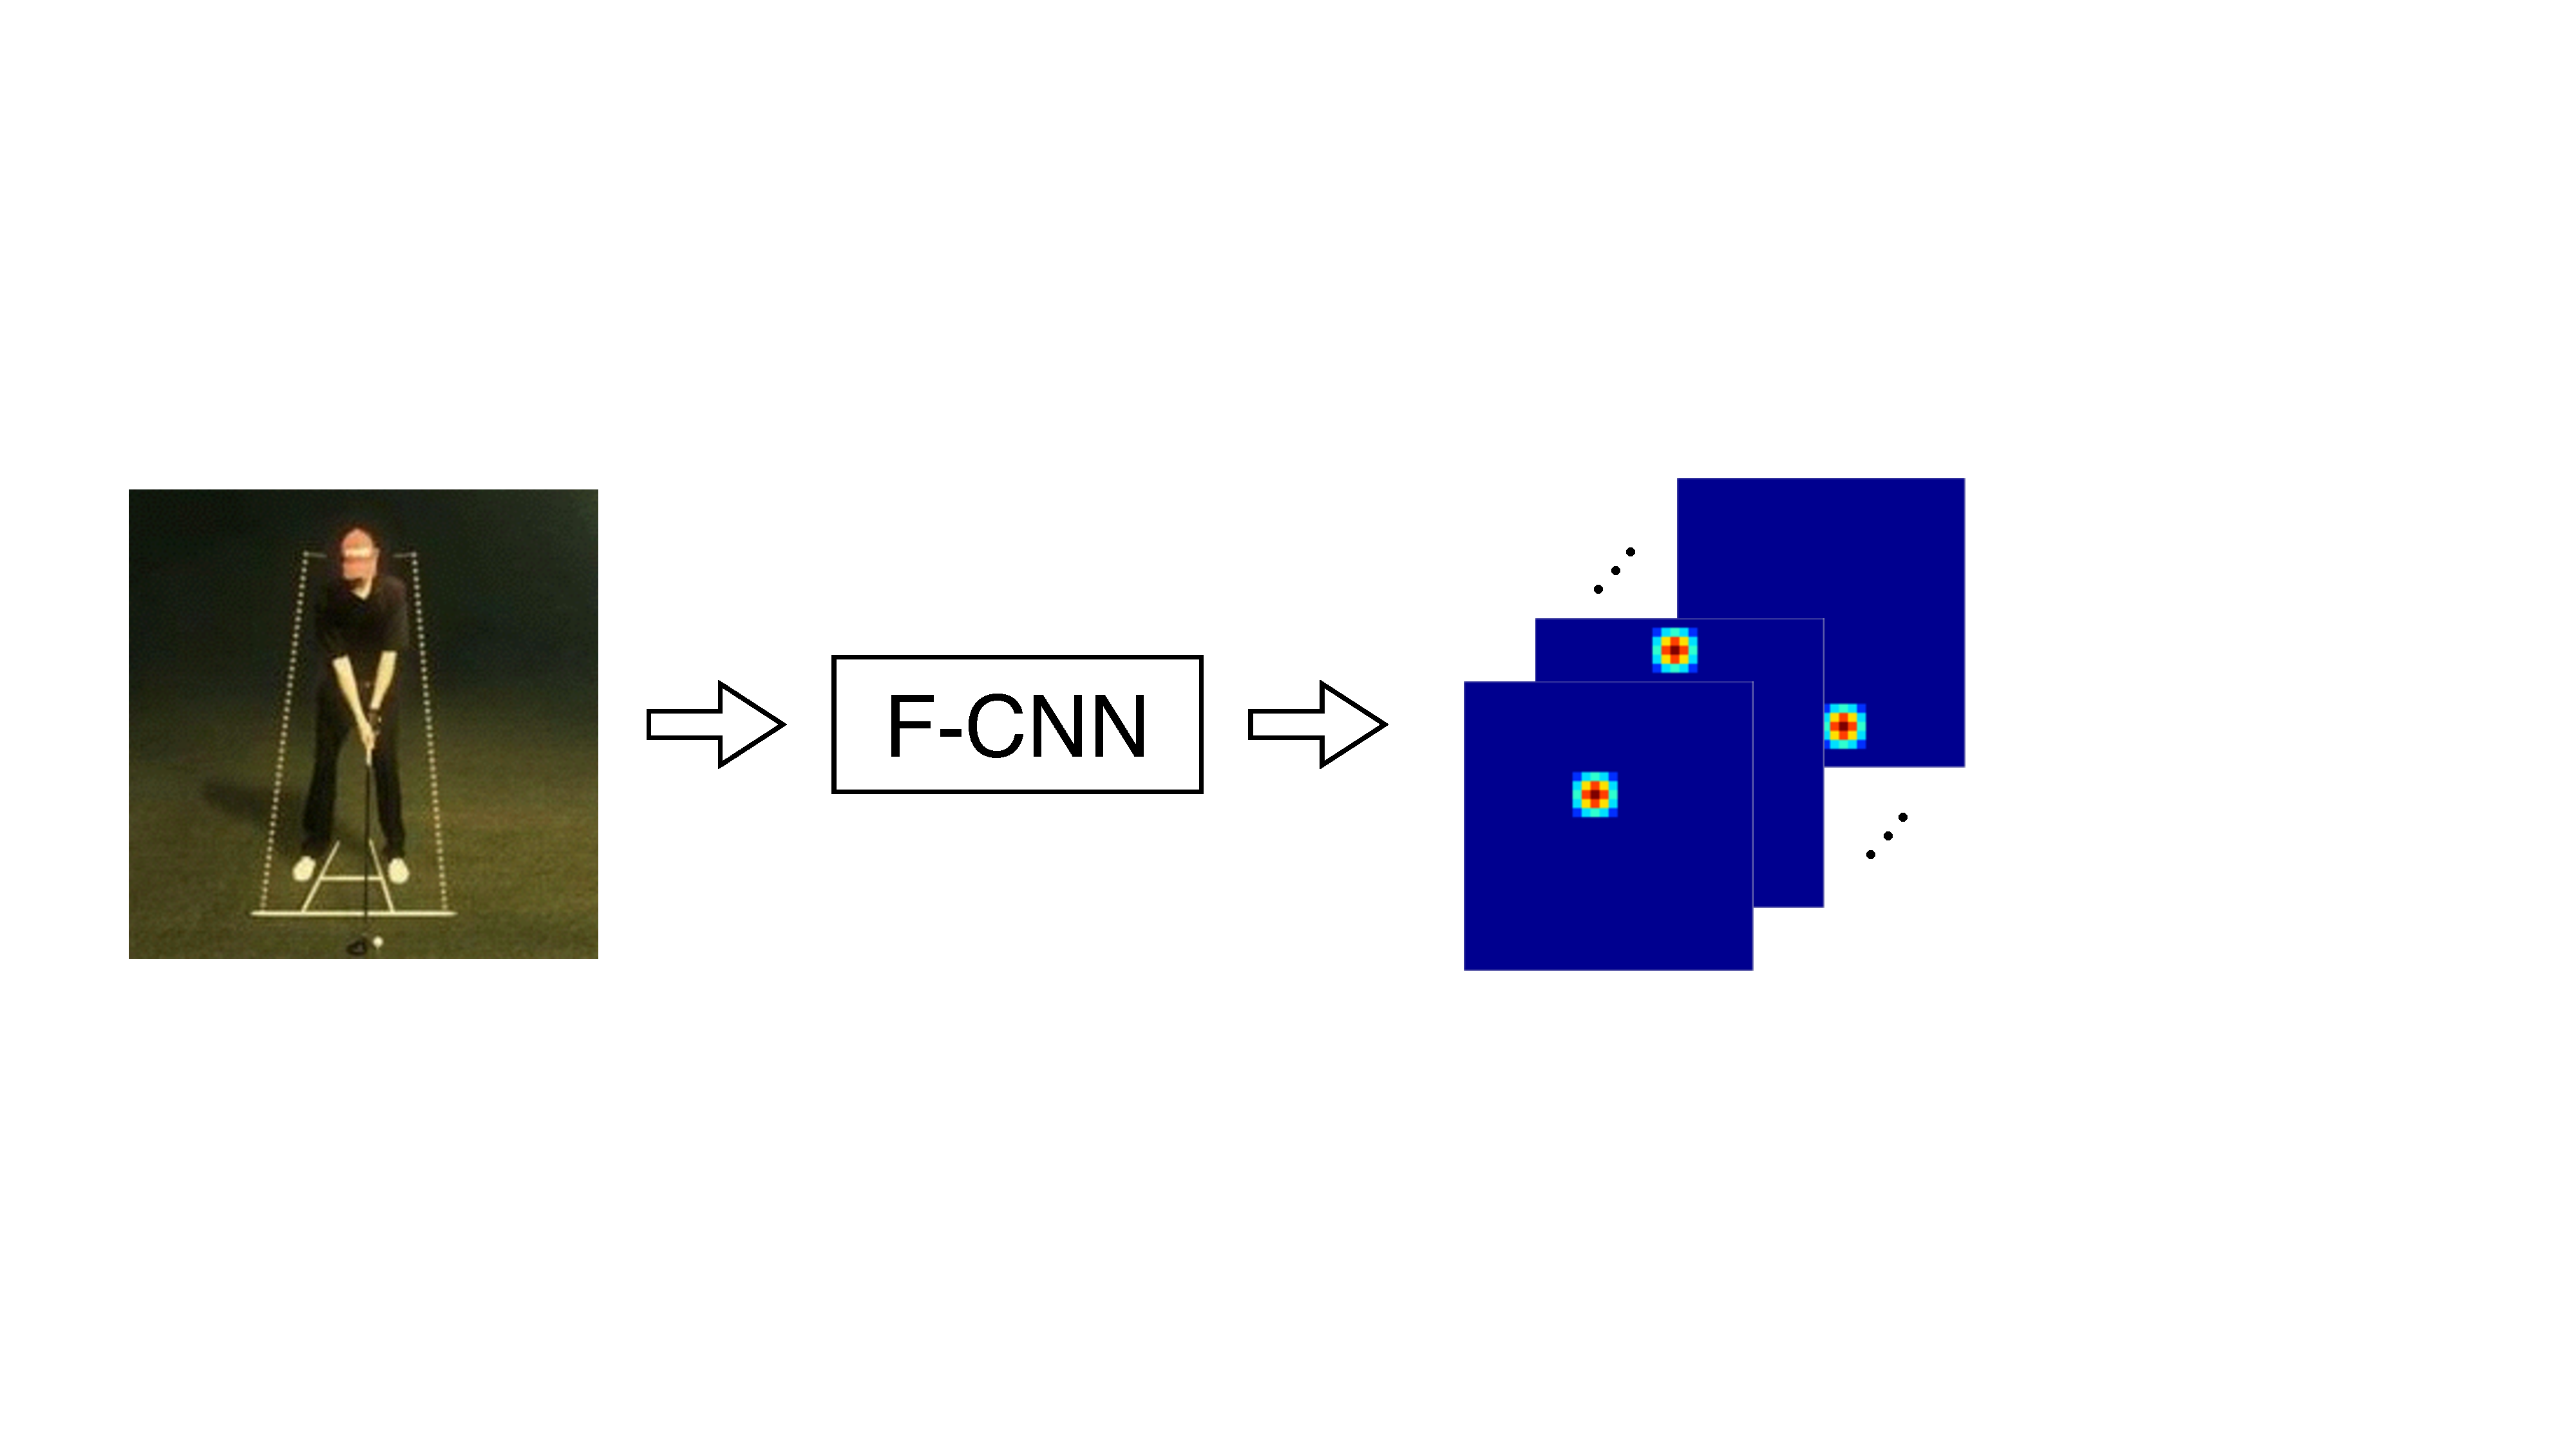
\includegraphics[width=\linewidth]{figures/cnn1.pdf}
  \caption{CNN-based 2D joint regressor. The network is a fully convolutional neural network (F-CNN). The input is an image and the output is a multi-channel heat map with each channel capturing the spatial uncertainty distribution of a joint. }\label{fig:cnn}
\end{figure}

